%% Journal of Chemical Information and Modeling
\documentclass[journal=jcisd8,manuscript=article]{achemso}

\usepackage[T1]{fontenc}
\usepackage{amsmath,amssymb}
\usepackage{booktabs}
\usepackage{graphicx}

\SectionNumbersOn

\author{Talha Kırca}
\email{talhakirca@kmu.edu.tr}
\affiliation{Department of Data Science and Analytics, Karamanoğlu Mehmetbey University, 70200 Karaman, Türkiye}
\author{Hasan Yıldırım}
\affiliation{Department of Data Science and Analytics, Karamanoğlu Mehmetbey University, 70200 Karaman, Türkiye}
\author{Merve Görgülü}
\affiliation{Department of Data Science and Analytics, Karamanoğlu Mehmetbey University, 70200 Karaman, Türkiye}

\title[Graph Network Attributions Track Atom Degree]
{Graph Network Attributions Track Atom Degree Before Training}

\keywords{Ames mutagenicity, graph neural networks, explainable artificial intelligence, attribution, negative controls, evaluation protocol}

\begin{document}

\begin{tocentry}
% ACS limits the graphic to 3.25 in by 1.75 in; the source figure is taller than
% that, so the height is capped and the aspect ratio preserved.
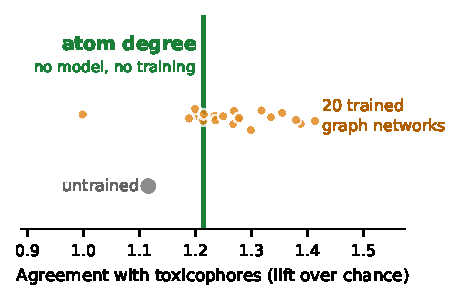
\includegraphics[width=\linewidth,height=1.7in,keepaspectratio]{figures/fig_toc.pdf}
\end{tocentry}

\begin{abstract}
Testing whether a graph neural network's attributions reflect learned chemistry requires a
reference that has learned nothing and is still worth beating. Ranking atoms by degree needs
no model and no training, and on the Ames endpoint it separates toxicophore atoms from the
rest at an area under the ROC curve of $0.580$, against $0.492$ for a random ranking. Against
it, a trained GIN shows two effects of opposite sign that a single aggregate figure conceals:
on the heteroatom-centred alerts it exceeds the baseline by $+0.193$, and on the fused
aromatic systems that supply 62\% of the alert atoms it falls to chance, $-0.172$ below it.
Both survive correction, hold under three readings of that alert, and replicate in direction
on the lift scale on three partitions drawn with a corrected scaffold splitter. Aggregated
over the whole library the difference is small, and a single figure would report that a model
which has demonstrably learned part of this chemistry adds little. The choice of measure
matters as much: at the retained fraction of 30\% of atoms this literature uses, no
architecture exceeds the baseline at all, 87\% of what that fraction selects from a degree
ranking being decided by a tie. Five hundred random initialisations reproduce the
per-molecule behaviour of the degree ranking. We recommend that agreement be reported on a
threshold-free measure, across alert subsets, and against a pre-specified model-free
structural ranking.
\end{abstract}

\section{Introduction}

The Ames test remains the regulatory reference for bacterial mutagenicity, and predicting its
outcome computationally is among the oldest and best-populated tasks in cheminformatics. Two
claims travel with the graph-based approach to it. The first is that message-passing networks
outperform models built on fingerprints and trees. The second, and the one this paper is
about, is that when a graph model's attributions land on known toxicophores, the model has
learned that chemistry.

The second is an inference rather than an observation, and like any inference it stands or
falls on the control against which it is drawn. Suppose an attribution method places atoms
inside a structural alert more often than chance would. That excess may reflect what the
network learned during training. Equally, it may arise from the architecture and the
attribution rule acting together on molecular graphs, quite apart from anything the network
was taught. Telling the two apart is what a negative control is for.

The explainable-AI literature has recommended comparing against chance and against a
randomised model since Adebayo and co-workers set out their sanity checks.\cite{adebayo2018}
In the same work they made an observation that has travelled less well. Some saliency methods
produce maps closely resembling those of an edge detector, which is untrained and depends
only on the input, and a reader who takes the highlighted edges for an explanation is exposed
to confirmation bias. Later work found that the reading does not necessarily hold for
Integrated Gradients in the image setting.\cite{kokhlikyan2021} Cheminformatics has adopted the randomisation checks in various
forms,\cite{hartog2024,walter2024} but not the edge detector, and so not the idea of a
reference that requires no model at all.

Degree-based descriptors are of course not new to the field. The Randi\'c connectivity
index\cite{randic1975} and the Zagreb indices\cite{gutman1972} are sums over atom degrees and
have served as elementary baselines in structure--property modelling for half a century. What
has not been done, as far as we can establish, is to use a degree ranking as the reference
against which an \emph{attribution} is judged.

We construct that reference for molecules. Atom degree is available from the molecular graph
in one line, needs no training, and can be scored against the same alerts and the same
overlap measure used to score attributions. Putting it beside the trained models changes what
can be concluded. On the Ames endpoint the degree ranking reaches $1.214\times$ chance
agreement, against $1.265 \pm 0.092$ for twenty trained GIN models, and it exceeds a
quarter of them outright. Five hundred randomly initialised networks reproduce its
per-molecule behaviour at a partial correlation of $0.57$, which identifies what the untrained
baseline has been measuring all along.

The accuracy comparison that usually accompanies such claims is revisited alongside, under a
cross-validation design adopted after we found a defect in our own earlier partitioning.
There the best classical model and the best graph model prove indistinguishable, and bond
features, the representational advantage most often claimed for graph models on molecules,
contribute nothing measurable.

\section{Related work}

Whether graph models outperform descriptor models on molecules has stayed open since
\citet{jiang2021} found the descriptor-based ones competitive with or superior to them
across benchmark tasks. Reported Ames performance
spans a wide range: \citet{thompson2025amesformer} report state-of-the-art results with graph
transformers, \citet{monem2025enhanced} and \citet{li2021mutagenpred} with convolutional
architectures. \citet{vantilborg2022} report descriptor models outperforming graph models on
activity-cliff benchmarks, a result of the same shape as ours on this endpoint. The spread
between such reports is wide enough that protocol differences must contribute to it, and Section~\ref{sec:partition} quantifies one
such difference in our own earlier design.

The evaluation protocol is itself a confound, and the field has long known it. Permuting the
response and refitting is established practice: y-randomisation has
been standard QSAR validation since Golbraikh and Tropsha\cite{golbraikh2002} and the
systematic treatment of Rücker and co-workers,\cite{rucker2007} a decade before the
sanity-check literature we draw on. That reported gains can be artefacts of unequal tuning is
established outside chemistry.
\citet{dacrema2019} found most neural recommendation methods outperformed by properly tuned
classical baselines, and \citet{musgrave2020} reached the same conclusion for deep metric
learning. Closest to the present setting, \citet{errica2020} found a structure-agnostic
baseline competitive with graph networks across graph-classification benchmarks under a
protocol critique much like ours. \citet{demsar2006} set out the machinery for comparing classifiers over multiple
datasets, which assumes those datasets are independent, an assumption we examine in our own
earlier design. Within cheminformatics the optimism of random splitting is
acknowledged,\cite{sheridan2013,wu2018moleculenet} though rarely quantified against a matched
number of scaffold partitions.

How an explanation should be evaluated has been approached from several directions.
\citet{mccloskey2019attribution} used tasks with known binding logic to test whether
attributions recover it, and \citet{matveieva2021} assembled datasets with known ground-truth
interpretations for the same purpose;
\citet{sanchez2020evaluating} and \citet{agarwal2023graphxai} extended systematic evaluation
to graph models, and \citet{amara2022graphframex} catalogued fidelity metrics.
\citet{rao2022quantitative} and \citet{wu2023sme} evaluated attributions against chemical
substructures, \citet{jimenezluna2021coloring} against atom-colouring schemes, a practice set out by
\citet{sheridan2019}. Closest to our
setting, \citet{walter2024} compared model explanations with expert-derived alerts for Ames
mutagenicity and \citet{hartog2024} found alert importance largely model-independent,
including for randomised models. \citet{faber2021comparing} raised the complementary caution
that a mismatch with ground truth may indicate the model does not use those features rather
than that the explanation is wrong. \citet{khasanova2026} report that attribution quality
degrades sharply below a threshold of predictive performance. Outside chemistry the same
concern has been pressed harder. \citet{hooker2019} found several attribution methods unable
to beat a random ranking under a retraining-based control, and \citet{sixt2020} showed that
a family of modified backpropagation methods produces attributions determined substantially
by the architecture, not by the learned weights. The latter is the closest precedent
for the mechanism we report here. What none of this work supplies is a reference that
requires no model.

Message-passing networks are known to treat nodes of different degree differently, a bias
documented on node-level tasks. In node classification,
performance is systematically better for high-degree
nodes,\cite{subramonian2024,ju2023} and \citet{subramonian2024} trace the effect to several
properties that covary with degree. Our observation is different in kind: on a graph-level molecular task, the
\emph{attributions} of a network track atom degree, and they do so before the network is
trained. The two are consistent, and the first makes the second less surprising, but neither
implies the other.

\section{Methods}

\subsection{Data and partitioning}

Structures come from the Ames benchmark distributed with the Therapeutics Data
Commons,\cite{huang2021} which takes its data from the compilation of Xu and
co-workers.\cite{xu2012} SMILES were canonicalised with RDKit\cite{rdkit} and duplicates
identified on the canonical SMILES string. No compound failed to parse, carried a
contradictory duplicate label, or duplicated another, leaving 7,255 compounds of which 54.5\%
are mutagenic. We applied no further standardisation: salts were not stripped and neither
tautomers nor charge states were normalised. Two checks bound what that omission can cost
here. No record in the dataset contains more than one covalent component, so no counter-ion
contributes atoms to $|\mathcal{A}|$. And every nitro group in the canonical SMILES is written
in the charge-separated form the aromatic nitro pattern requires, with no occurrence of the
neutral pentavalent alternative, so that pattern loses no match to representation. Patterns
that specify charge or a particular tautomer remain sensitive to representation in general,
and a differently curated source could behave differently.

Two designs are used. For the comparison between models, Bemis--Murcko
scaffolds\cite{bemis1996} are dealt into ten folds, each of which serves once as the test
set, so every compound receives exactly one prediction from a model that never saw its
scaffold. Assignment is by scaffold, so no scaffold appears in both parts of any fold, and a
scaffold-disjoint tenth of each fold's training portion is held out for early stopping.

The partition used for the attribution analyses was drawn with the size-ordered rule
described in Section~\ref{sec:partition}, before we identified its defect. That same section
repeats the analysis on three partitions drawn with the corrected rule.

The attribution analyses are carried out on GIN. It was designated before the
cross-validation was run, when a fifteen-partition benchmark placed it ahead of the other two
architectures; the cross-validation reported below later placed GAT ahead. We did not revise
the choice, and Section~\ref{sec:arch} reports all three architectures for the central
comparison. These analyses require one designated model, and for it a single scaffold
partition is drawn with a seed disjoint from the folds, giving 5,804 training, 725 validation
and 726 test compounds. Scaffold partitioning does not preserve the mutagenic fraction: the
training set is 55.6\% mutagenic and the test set 46.3\%.

An earlier version of this work compared models over fifteen independently drawn scaffold
partitions. That design proved defective for reasons reported in
Section~\ref{sec:partition}, and cross-validation replaces it.

\subsection{Models and training}

Circular fingerprints are 2048-bit Morgan fingerprints of radius 2.\cite{rogers2010} RDKit
two-dimensional descriptors provide a second, physicochemical view of the same molecules.
Molecular graphs carry a 24-dimensional atom feature vector (one-hot element and
hybridisation, degree, formal charge, aromaticity, hydrogen count, ring membership) and a
6-dimensional bond vector (bond order, aromaticity, conjugation, ring membership). Degree
throughout this work is the number of explicit heavy-atom neighbours, RDKit's
\texttt{GetDegree}, with hydrogens implicit.

Six models are compared: XGBoost\cite{chen2016} and a random forest on fingerprints, XGBoost
on descriptors, and GCN,\cite{kipf2017} GIN\cite{xu2019} and GAT\cite{velickovic2018}
implemented in PyTorch Geometric.\cite{fey2019} A logistic regression on fingerprints
provides a linear reference. GIN and GAT consume bond features; GCN operates on connectivity
alone. Ablated variants of GIN and GAT without bond features receive their own hyperparameter
search over the same space and budget.


Hyperparameters were searched once on the designated partition with Optuna,\cite{akiba2019}
under a fixed budget of one hundred trials per model, selected on validation ROC-AUC, and the selected configurations were
reused in the cross-validation. The search was therefore not nested inside the folds, and
Section~\ref{sec:accuracy} measures what that cost. Graph models were trained with an
unweighted loss, early stopping on validation ROC-AUC and a fixed epoch ceiling; predictions
are means over three training seeds. Search spaces, selected configurations and wall-clock
budgets are in the Supporting Information.

\subsection{Attribution protocol}

Toxicophores are matched with SMARTS patterns drawn from the alerts of Kazius and
co-workers,\cite{kazius2005} who derived 29. We encoded the 18 for which a single
unambiguous SMARTS expression could be written without inferring bounds the original does not
state; the remaining 11 describe classes whose translation into one pattern would have
required choices of our own. The 18 were fixed before any agreement was computed. Published SMARTS for these alerts are
available through ToxAlerts,\cite{sushko2012} and using them would remove one of our choices
from the analysis. For seventeen of the eighteen the question is narrow, since the patterns
are small and admit little latitude. For the fused-aromatic alert it is not. Our pattern is a
naphthalene substructure query, so it matches any molecule containing two fused aromatic
rings, phenanthrene and benzo[a]pyrene among them; what it cannot do is distinguish a bare
naphthalene from a bay-region system, and Kazius and co-workers describe the alert without specifying it. We therefore test that
alert by ring perception instead, under three readings, and report the sensitivity instead of substituting one fixed encoding for another (Supporting Information). Four of
them match no molecule in the evaluation set and a fifth matches one, so the library that
does any work here consists of 14 patterns: one matching fused aromatic systems and 13
centred on heteroatoms. All 18 are listed with their coverage in the Supporting Information. The
evaluation set is every test compound that is mutagenic and contains at least one match
without being matched in its entirety, giving 237 molecules from the 336 mutagenic test
compounds; 74 matched no alert and 25 were matched throughout.

For a molecule with atom set $\mathcal{A}$, toxicophore atoms $\mathcal{T}$ and the $k$ most
highly ranked atoms $\mathcal{S}_k$, where $k$ is 30\% of $|\mathcal{A}|$, the observed
overlap is $o = |\mathcal{S}_k \cap \mathcal{T}| / |\mathcal{S}_k|$ and the chance overlap is
$c = |\mathcal{T}| / |\mathcal{A}|$. The reported agreement is the ratio of the two means
across molecules,

\begin{equation}
\label{eq:lift}
\mathrm{lift} \;=\;
\frac{\frac{1}{n}\sum_{i=1}^{n} o_i}{\frac{1}{n}\sum_{i=1}^{n} c_i},
\end{equation}

not the mean of per-molecule ratios, which is unstable for molecules with few
toxicophore atoms. Ties are broken at random, not by atom index, and every ranking is
scored over 200 independent tie-breaks, because several of the rankings compared below are
binary and leave large numbers of ties.

A lift of one indicates agreement no better than selecting atoms at random. The attainable
maximum is not $1/\bar{c}$: a molecule with fewer alert atoms than the selection retains
forces even a perfect ranking to fill the remaining positions from outside any alert. We
therefore measure the ceiling from a ranking that places every alert atom first, obtaining
$1.914$ at the reference fraction against a nominal bound of $2.293$. Since the ceiling
depends on both the retained fraction and the alert library, every figure reported as a
percentage of it states which ceiling applies.

Four attribution methods are applied to trained graph models: Integrated
Gradients\cite{sundararajan2017} over a 32-step path from a zero baseline, Gradient $\times$
Input, Saliency, and GNNExplainer.\cite{ying2019} TreeSHAP values\cite{lundberg2020} for the
fingerprint model are distributed to atoms through the environments each bit encodes,
following the similarity-map construction of \citet{riniker2013},
dividing each bit's contribution equally among its environments and among the atoms of each.
Gradient attributions are aggregated as an absolute sum over feature dimensions and SHAP
values read as signed contributions; both conventions are evaluated for both and reported.

\subsection{Model-free baselines and negative controls}

Because atom degree is itself one of the atom features, two reduced encodings were also
prepared, one omitting degree and one omitting degree together with hydrogen count, which is
its complement at fixed valence. Networks were fitted and attributions computed under both,
so that an association arising from the encoding can be separated from one arising from
message passing.

Eleven rankings are computed from the molecular graph alone. They are atom degree,
heteroatom status, number of heteroatom neighbours, aromaticity, ring membership, hydrogen
count, absolute formal charge, the disjunction of heteroatom status with heteroatom
neighbours, the sum of heteroatom status and normalised degree, absolute deviation of degree
from the molecular mean, and element rarity within the molecule.

Atom degree is the primary baseline. It was chosen after the eleven rankings were scored, on
the screen reported in Section~\ref{sec:regimes}, and we say so instead of claiming otherwise. What recommends it is that it is the simplest of the eleven, it requires no choice
of parameter, a mechanism for it was available in advance, and it is the only one whose
interval lies above chance under all three regimes. The choice is defensible on those grounds,
but it was not fixed in advance and we do not present it as such. What the mechanism
anticipated is that the dominant pattern in the alert library matches fused aromatic systems,
whose atoms are of high degree by construction. The other ten serve as a sensitivity panel. Taking
the strongest of a panel as the reference would bias the comparison in the direction of this
paper's own critical conclusion, so where the panel maximum differs from degree we report it
as such and state the direction of the bias.


Four controls bound what agreement can be reached without the thing being claimed: a random
atom ranking, an untrained network, a network fitted to permuted labels, and a shuffle of the
attribution scores within each molecule. Each is a distribution, not a point, drawn
over initialisations or over shuffles, and each is compared with the trained models in the
same paired design. Full definitions are in the Supporting Information.

\subsection{Statistics and reproducibility}

Models are compared on the out-of-fold predictions by a bootstrap over compounds with 10,000
resamples, drawn jointly so that every model sees the same replicate. Where several models
are tested against the same reference, $p$-values are corrected by Holm's procedure. Paired
comparisons at the level of molecules use the Wilcoxon signed-rank test with the
matched-pairs rank-biserial correlation as effect size, and intervals on the effect of
training resample molecules and models together.


The pipeline is released as notebooks with all random seeds fixed. Model weights, the raw
atom-level attributions of the graph models and the fold assignments are retained; a manifest
records which stage produced each result file, and a companion file lists every quantity
quoted in this text. The atom-level TreeSHAP values were not kept, which is why the fingerprint
model appears on the lift scale alone.

\section{Results}

Supporting checks are reported inside the finding each one bears on. The decision rule that
governs every comparison below is stated first.

\subsection{Decision rule}
\label{sec:rules}

Four comparisons in this paper are made against the degree ranking, and they do not form one
family. Grouping them is a choice, and we fixed it before the corrected values were computed:
the five ranking-AUROC comparisons form one family, the three specificity tests another, the
three cells at the smallest retained fraction a third, and the six cells of the two reduced
regimes a fourth. Holm is applied within each. The panel of eleven structural rankings carries no
correction: it is a screen that selected the baseline, not a test. Nor does the sweep
at the four larger fractions, for a reason worth stating. The claim drawn from those twelve
cells is that no architecture exceeds the baseline, and a correction can only make a claim of
absence harder to overturn. Leaving them uncorrected is the conservative reading for
what is claimed from them. The full rule, with test counts read from the tables
themselves, not stated, is in the Supporting Information.

\subsection{A degree ranking is a strong reference, and untrained networks already track it}
\label{sec:arch}

\begin{figure}[htbp]
\centering
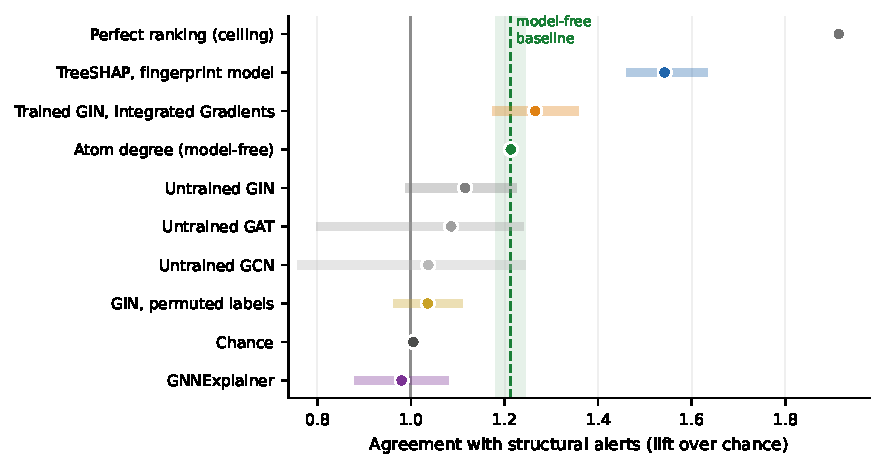
\includegraphics[width=0.72\textwidth]{figures/fig01_ladder.pdf}
\caption{Agreement with structural alerts on the 237 evaluation molecules. Bar conventions
differ by arm and are not comparable to one another: standard deviation across models for the
trained and permuted arms, the central 95\% of 500 draws for the untrained arms, and a
bootstrap over molecules for TreeSHAP. The dashed line is the model-free baseline and the
shaded band its bootstrap interval over molecules, which is the interval the comparisons in
this paper use.}
\label{fig:ladder}
\end{figure}

On the 237 evaluation molecules a ranking by atom degree agrees with the alerts at
$1.214 \pm 0.013$ times chance, the spread being over tie-breaks, not over models,
since the ranking is deterministic. Twenty independently trained GIN models reach
$1.265 \pm 0.092$ with Integrated Gradients, spanning $0.999$ to $1.413$
(Figure~\ref{fig:ladder}). Saliency behaves almost identically at
$1.269 \pm 0.101$, and Gradient $\times$ Input reaches $1.189 \pm 0.091$.

Whether that difference is resolvable depends on how the baseline is treated. We call a
difference resolved when its interval excludes zero, and unresolved otherwise; throughout this
paper that is what the word means.

Treated as a fixed number, the baseline resolves the difference: a one-sample test against
$1.214$ gives $p = 0.040$ for GIN after correction. But $1.214$ is itself estimated from the
same 237 molecules, with a bootstrap interval of $1.183$ to $1.243$, and a comparison that
ignores that reports an interval $1.6$ times narrower. The cost is not only the understated
reference: a one-sample test against a constant excludes the molecule axis altogether, and on
these data that axis is the wider of the two.

Resampling molecules and models together, and taking the difference within each replicate, no
architecture exceeds the baseline on this measure (Table~\ref{tab:paired}): GIN differs by
$+0.052$ ($-0.014$ to $+0.119$) and GAT by $-0.011$ ($-0.046$ to $+0.025$). GCN falls below
it by $-0.061$, with an interval that excludes zero before correction but not after
($p = 0.077$ under Holm across the three tests).

\begin{table}[htbp]
\centering
\caption{Each architecture against the model-free baseline, with molecules and models resampled together so that the uncertainty of the reference is carried. The last column repeats the same comparison with the baseline treated as a fixed number.}
\label{tab:paired}
\small
\setlength{\tabcolsep}{4pt}
\begin{tabular}{lcccc}
\toprule
Architecture & $\Delta$ lift & 95\% CI & $p$ (Holm) & Fixed-reference $p$ \\
\midrule
GIN & +0.0518 & -0.014 to +0.119 & 0.242 & 0.040 \\
GAT & -0.0112 & -0.046 to +0.025 & 0.537 & 0.365 \\
GCN & -0.0606 & -0.114 to -0.008 & 0.077 & 0.007 \\
\bottomrule
\end{tabular}
\begin{flushleft}\footnotesize No architecture is separated from the baseline once the reference is allowed to vary. Treating it as fixed narrows the interval by a factor of about two and produces the separations in the last column.\end{flushleft}
\end{table}


The same comparison for all three architectures is shown in the Supporting Information.

Whether agreement tracks predictive performance cannot be settled at this sample size. The
sixty models span $0.751$ to $0.803$ in test ROC-AUC, and within each architecture the
correlation between agreement and performance is $0.26$ for GIN (95\% CI $-0.21$ to $0.63$),
$0.27$ for GAT and $0.29$ for GCN, every interval containing zero
(Supporting Information). The three cannot be combined: the same 237 molecules are scored
against the same alert library in all three, and their per-molecule agreements correlate with
the degree ranking at $0.82$, $0.96$ and $0.89$. Pooling the sixty models gives $r = 0.39$,
confounded with architecture identity since GIN has both the highest mean performance and the
highest agreement and GCN the lowest of each. We draw no conclusion from either figure.

Five hundred randomly initialised GIN networks give a mean agreement of $1.116 \pm 0.059$,
with the central 95\% of draws spanning $0.989$ to $1.226$. Two further architectures behave
similarly with wider spread, GCN at $1.037 \pm 0.141$ and GAT at $1.086 \pm 0.125$.

Two intervals should be kept apart here. The spread of the draws describes what a single
initialisation may return, and for all three architectures it includes chance: an individual
untrained network is not reliably above it. The interval on the mean is narrower and for all
three it excludes chance. Resampling draws alone gives $[1.110, 1.121]$ for GIN, $[1.075, 1.097]$ for GAT and
$[1.025, 1.049]$ for GCN. Resampling molecules with them, which is the comparison argued for
above, widens these to $[1.074, 1.157]$, $[1.062, 1.111]$ and $[1.008, 1.064]$. The draws
themselves span $0.885$ to $1.275$ for GIN, so a single untrained network is too noisy to
serve as a reference. The conclusion
is unchanged, but the widening is not uniform: about twofold for GAT and GCN and eightfold for
GIN, whose draw-to-draw standard deviation is $0.059$ against $0.125$ and $0.141$. The
architecture with the least variable initialisations is the one whose interval widens most
once molecules are resampled with them.

The three control distributions differ from the untrained networks as distributions, not merely as means (permutation $p < 0.001$ in each case), so the untrained network is not
interchangeable with a random ranking, a degree ranking or a shuffled attribution
(Supporting Information).

Compared molecule by molecule, an untrained network tracks the degree ranking closely. For GIN
the per-molecule agreements correlate at $0.943$, and at $0.567$ once each molecule's chance
coverage is removed. The second figure is the one that carries the claim: on the raw scale a
random ranking already reaches $0.807$, against $-0.033$ once the shared bound is removed, so
most of the raw correlation reflects that bound, not agreement (Supporting
Information). The within-molecule Spearman correlation over 200 random initialisations is
$0.68$.

The association survives training. The within-molecule correlation falls to a mean of $0.43$
across the twenty trained models without disappearing, and at the level of per-molecule
agreement the trained architectures track the degree ranking at $0.824$ for GIN, $0.955$ for
GAT and $0.889$ for GCN (Figure~\ref{fig:mechanism}). It is weakened but not displaced by what
the model learns.

\begin{figure}[htbp]
\centering
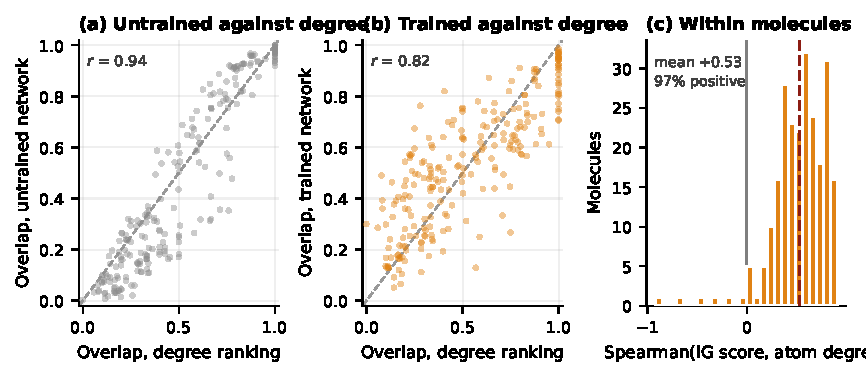
\includegraphics[width=0.98\textwidth]{figures/fig02_mechanism.pdf}
\caption{(a, b) Per-molecule agreement of the untrained and trained networks against the
degree ranking; the diagonal marks equality. (c) Within-molecule association between
Integrated Gradients scores and atom degree, one value per evaluation molecule.}
\label{fig:mechanism}
\end{figure}

Following training epoch by epoch across five runs, agreement rises from $1.110$ before
training to a plateau near $1.19$ by the twentieth epoch and stays there. Validation ROC-AUC
continues to climb from $0.73$ to $0.83$. Whatever the later epochs add to prediction, they do
not add agreement with the alerts.

\subsection{The retained-fraction measure is dominated by tie-breaking}
\label{sec:ties}

TreeSHAP on the fingerprint model reaches $1.542$ ($1.462$ to $1.633$), well clear of the
baseline and of every gradient method on a graph model, so what the tie-breaking result
describes is message passing with gradients, not attribution in general. The comparison
differs on two axes at once, the attribution rule and the representation, so neither can be
credited alone; running Integrated Gradients on the fingerprint model separates the two
and is reported in the Supporting Information. And GNNExplainer, measured on five trained
models under three regularisation settings, agrees with the alerts at $0.970 \pm 0.100$ at the
default setting and does not exceed chance under any of the three, so a mask-based explainer
adds nothing here that the gradient methods do not.

Both of these comparisons are made at a retained fraction of the ranking, and that choice
turns out to carry more than we assumed. Atom degree takes five distinct values across this
dataset, and in practice four, since the highest occurs on a single atom in the whole
library; within any one molecule there are fewer still. Most of the retained set is therefore
filled not by the ranking but by breaking ties at random within a degree level. Measured directly, 87\% of the
top-30\% set selected by degree is decided by a tie at the cut, against about 19\% for the
attributions (Supporting Information). The lift measure has been comparing a largely arbitrary
selection with an informative one.

Scoring alert membership by the attribution and taking the area under the ROC curve removes
the threshold and the tie-breaking together: it uses the whole ranking and resolves ties by
the mid-rank convention. We call this the ranking AUROC, to keep it apart from the lift of
Equation~\ref{eq:lift}; agreement with the alerts is the quantity, and the two are scales for
it. On the ranking AUROC the degree ranking reaches $0.580$ and twenty random
rankings $0.492$, so the measure behaves as it should. Twenty GIN models reach $0.637$, a
difference of $+0.056$ ($+0.019$ to $+0.093$) under the same paired resampling. Saliency
reaches $0.644$, $+0.063$ ($+0.024$ to $+0.102$). Both survive Holm correction across the
five attribution comparisons, at $p = 0.014$ and $p = 0.009$; GAT, GCN and Gradient
$\times$ Input do not separate from the baseline (Table~\ref{tab:auroc_p}).

\begin{table}[htbp]
\centering
\caption{Agreement on the threshold-free measure, with bootstrap $p$-values and Holm correction across the five attribution comparisons.}
\label{tab:auroc_p}
\footnotesize
\setlength{\tabcolsep}{4pt}
\begin{tabular}{lccccc}
\toprule
Ranking & $n$ & $\Delta$ vs.\ degree & 95\% CI & $p$ & $p$ (Holm) \\
\midrule
random ranking & 20 & -0.087$^{*}$ & -0.106 to -0.068 & 0.0002 & -- \\
trained GIN, IG & 20 & +0.056$^{*}$ & +0.019 to +0.093 & 0.0036 & 0.0144 \\
trained GAT, IG & 20 & +0.015 & -0.007 to +0.037 & 0.1680 & 0.3360 \\
trained GCN, IG & 20 & +0.018 & -0.013 to +0.048 & 0.2538 & 0.3360 \\
Gradient x Input & 20 & +0.030 & -0.003 to +0.063 & 0.0766 & 0.2298 \\
Saliency & 20 & +0.063$^{*}$ & +0.024 to +0.102 & 0.0018 & 0.0090 \\
\bottomrule
\end{tabular}
\begin{flushleft}\footnotesize An asterisk marks a comparison resolved at 0.05 after correction. The random ranking is a control on the measure rather than a claim about a model and carries no corrected value; twenty independent rankings were drawn for it, as twenty models were fitted for each architecture.\end{flushleft}
\end{table}


The two scales therefore disagree, and the disagreement is informative, not awkward.
At a retained fraction of 30\% the trained models are indistinguishable from a ranking whose
own selection is seven-eighths arbitrary; on the whole ranking, one architecture and one
gradient method are ahead of it. We report the ranking-AUROC comparison as the primary one
and the lift comparison as a sensitivity analysis, since the second inherits a choice the
first does not. TreeSHAP cannot be placed on this scale because its atom-level scores were
not retained, so the comparison between the two model families remains a lift comparison.

The comparison also depends on how much of the ranking is retained
(Supporting Information). Among the ten per cent of atoms a model attributes most strongly, GIN exceeds the degree
ranking by $+0.229$ ($+0.118$ to $+0.354$) and GAT by $+0.136$ ($+0.063$ to $+0.215$). Both
survive Holm across that subfamily at $p = 0.001$, under the rule of
Section~\ref{sec:rules}. The difference falls as more atoms are
retained and is smallest near the reference fraction of $0.30$, which is where we set it. At
the top of the ranking the trained models lead the baseline; averaged over a third of the
atoms they do not.


Expressed as a share, the baseline accounts for 81\% of GIN's above-chance signal
($64$--$107$\%), 106\% of GAT's and 140\% of GCN's. Only for GCN does the interval lie
entirely above 100\%, which would mean the model-free ranking accounts for the whole of what
the trained model achieves; for GAT the point estimate exceeds it but the interval does not,
and for GIN neither does (Supporting Information).

\subsection{One aggregate figure averages two effects of opposite sign}
\label{sec:regimes}

The alert library is not homogeneous, and the imbalance is severe. One of the eighteen
patterns matches fused aromatic systems and is composed entirely of carbon. It matches 97 of
the 237 evaluation molecules and supplies 61.8\% of all alert atoms there. Over the 2,884
mutagenic compounds that satisfy the same partial-match rule the share is 46.5\%, the
difference following from the absence of acyclic compounds from any evaluation set
(Section~\ref{sec:partition}). The 13 heteroatom-centred patterns that match anything share the
rest.

Scored on its own it would admit seven further compounds that the full library matched in
their entirety, giving 104 molecules. We hold the evaluation set fixed at the 237 instead, so
that the three regimes decompose one set of molecules rather than three, and the fused
aromatic regime is the 97 of them the pattern matches. Scored separately, the two groups reward opposite
rankings (Figure~\ref{fig:regimes}). A flag marking heteroatoms and their neighbours reaches
$1.735$ with the aromatic pattern removed and $0.603$ with it alone. An aromaticity flag does
the reverse, $0.519$ and $1.297$. Resampling the molecules in each regime, atom degree is the
only one of the eleven whose interval lies above chance under all three, at $1.214$
$[1.184, 1.245]$, $1.278$ $[1.223, 1.334]$ and $1.162$ $[1.127, 1.198]$. Every other ranking
either includes chance in at least one regime or falls below it. The thirty-three intervals
are a screen that fixed the choice of baseline, not thirty-three inferential tests: they carry
no correction, and the regimes are nested, not independent, the full library being the union
of the other two.

The screen was applied on one partition, and the ranking it selected became the reference for
every comparison on those same molecules. Repeated on the three partitions of
Section~\ref{sec:partition} it returns atom degree each time (Supporting Information), so the
selection rule transports beyond the partition that produced it.


\begin{figure}[htbp]
\centering
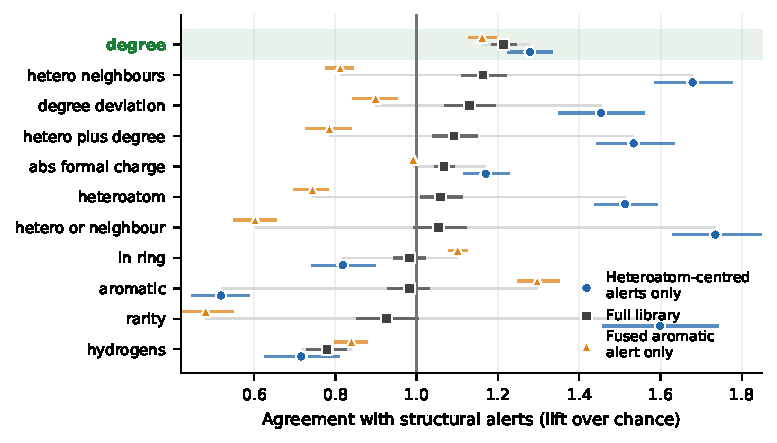
\includegraphics[width=0.78\textwidth]{figures/fig03_regimes.pdf}
\caption{Structural rankings under three regimes of the alert library, with intervals from
10,000 resamples of the molecules. Atom degree is the only ranking whose interval excludes
chance under all three; the thirty-three intervals are a screen over a panel and carry no
correction for multiplicity, and the regimes are nested, not independent.}
\label{fig:regimes}
\end{figure}

Degree is not the panel maximum under any regime: with the fused pattern removed the maximum
is $1.735$ against degree's $1.278$. What makes degree usable as a reference is that it alone
stays above chance under all three, and choosing the maximum instead would raise the reference
and strengthen this paper's own critical conclusion, so the choice made here is the
conservative one.

Two claims should be kept apart here, because they do not generalise alike. That the
attributions of a graph network track atom degree is a property of the model, established by
the within-molecule association and by the correlation with the untrained networks, and it
does not depend on the alert library at all. That atom degree is the best available
model-free baseline is a property of this library, which mixes two opposed regimes in a
particular proportion; degree wins because it is mediocre in both, not strong in either. A library weighted differently, or a different endpoint, could well be better served
by another ranking. The recommendation to use a model-free baseline survives that change; the
recommendation to use degree specifically would have to be re-examined.

Scoring the trained models under each regime separately shows what the aggregate
conceals.

On the ranking AUROC, with the fused aromatic pattern removed so that the library
consists of the heteroatom-centred alerts that encode recognised mutagenicity chemistry, GIN
reaches $0.715$ against $0.522$ for the degree ranking, a difference of $+0.193$ ($+0.151$ to
$+0.232$). The baseline is close to chance in this regime, $0.522$ against $0.492$ for a
random ranking, so what GIN exceeds there is a weak reference, not a strong one. The
informative comparison in this regime is with chance itself, and GIN is well clear of it. With that pattern alone, GIN falls to $0.495$, which is chance, while the degree ranking
reaches $0.667$. The difference is $-0.172$ ($-0.234$ to $-0.109$). Both survive Holm across
the six cells of the two reduced regimes at $p = 0.001$, and neither GAT nor GCN resolves from
the baseline in either regime after correction (Table~\ref{tab:regime_auroc}).

\begin{table}[htbp]
\centering
\caption{The regime decomposition on the threshold-free measure. The full library reproduces the published values and is a control; Holm is applied across the six cells of the two reduced regimes.}
\label{tab:regime_auroc}
\footnotesize
\setlength{\tabcolsep}{4pt}
\begin{tabular}{llcccc}
\toprule
Regime & Ranking & AUROC & $\Delta$ & 95\% CI & Tie \\
\midrule
Full library ($n$ = 237) & Atom degree & 0.580 & -- & -- & 0.87 \\
 & trained GIN & 0.637 & +0.056 & +0.019 to +0.093 & 0.19 \\
 & trained GAT & 0.595 & +0.015 & -0.007 to +0.037 & 0.19 \\
 & trained GCN & 0.598 & +0.018 & -0.013 to +0.048 & 0.20 \\
Heteroatom alerts ($n$ = 174) & Atom degree & 0.522 & -- & -- & 0.82 \\
 & trained GIN & 0.715 & +0.193$^{*}$ & +0.151 to +0.232 & 0.20 \\
 & trained GAT & 0.563 & +0.040 & +0.003 to +0.077 & 0.20 \\
 & trained GCN & 0.502 & -0.020 & -0.066 to +0.026 & 0.21 \\
Fused aromatic only ($n$ = 97) & Atom degree & 0.667 & -- & -- & 0.97 \\
 & trained GIN & 0.495 & -0.172$^{*}$ & -0.234 to -0.109 & 0.16 \\
 & trained GAT & 0.628 & -0.039 & -0.100 to +0.018 & 0.16 \\
 & trained GCN & 0.712 & +0.044 & -0.008 to +0.100 & 0.16 \\
\bottomrule
\end{tabular}
\begin{flushleft}\footnotesize An asterisk marks a difference resolved after correction. The last column is the share of the top-30\% set that a tie at the cut decides. It is $0.97$ for the degree ranking under the fused aromatic alert against $0.82$ under the heteroatom alerts, so the lift measure was doing different work in the two regimes; the threshold-free measure does not depend on it.\end{flushleft}
\end{table}


The lift measure gives the same two signs, at $+0.442$ and $-0.231$, and is reported as a
sensitivity analysis (Supporting Information). The two measures disagree about where
the baseline itself is strong, and the tie fraction says why: under the fused aromatic alert
the degree ranking carries $0.97$, so almost the whole of its retained set is decided at the cut, not by the ranking, against $0.82$ under the heteroatom alerts. Lift is bounded by
each regime's chance coverage and the ranking AUROC is not, so the baseline reads as
stronger on the heteroatom alerts under the first and on the fused aromatic systems under the
second. The comparison between a model and the baseline is unaffected, being made within a
regime, but the two regimes are not comparable to each other on the lift scale.


This is the most informative result of the attribution analysis and the largest separation
from the baseline anywhere in it. GIN learns something the degree ranking does not, and fails
on the pattern that supplies most of the alert atoms; the two effects have opposite signs and
comparable magnitude, so the aggregate cancels. Without a model-free reference neither would
be visible. The Supporting Information shows the same comparison on individual molecules.

The mechanism is not specific to this endpoint. Because it needs neither labels nor an
alert library, the association between an untrained network's attributions and atom degree
can be measured on any set of molecules (Supporting Information). On 299 compounds drawn from a blood--brain barrier penetration dataset, the
within-molecule Spearman correlation over 200 random initialisations is $0.646$, positive in
99\% of molecules, against $0.685$ and 98\% on the Ames evaluation set.

Alert atoms matter only where they carry the endpoint. A ranking that favours fused aromatic
atoms would score well on any molecule containing them, whether or not they carry it, so the
comparison was repeated on the 168
non-mutagenic compounds of the evaluation set under a signed aggregation, which the Supporting
Information sets out in full. On the designated partition GIN's advantage over the baseline
is smaller where alert atoms do not carry the endpoint, by $-0.050$ ($-0.090$ to $-0.011$,
Holm $p = 0.037$ across the three architectures); GAT and GCN do not resolve.

It does not survive redrawing. On the three partitions of Section~\ref{sec:partition} the
difference is $-0.089$ ($-0.152$ to $-0.031$), $+0.011$ and $-0.014$; only the first excludes
zero and the second has the opposite sign (Supporting Information). The pre-specified reading for a sign
reversal on any partition was to withdraw the claim, and we withdraw it. What the designated
partition shows is that the check can be made and that it can come out positive; it does not
show that trained graph models discount alerts in context.


\subsection{Ordering scaffold groups by size does not give independent partitions}
\label{sec:partition}

An earlier version of this work compared models over fifteen scaffold partitions drawn
independently. Their test sets overlap at a mean Jaccard index of $0.634$, against the
$0.053$ expected of independent tenth-samples of the same pool. The fifteen together cover
937 of the 7,255 compounds, and the design carries the weight of $1.26$ effective independent
observations, not fifteen. We take the effective number as $k/(1 + (k-1)\rho)$, the
usual design effect, with $\rho$ estimated from the mean pairwise Jaccard $J$ as the shared
fraction $2J/(1+J)$. The intraclass correlation of the partition-level ROC-AUC values gives a
lower figure still, $1.02$, but it measures partition difficulty, not test-set overlap
(Supporting Information) (Figure~\ref{fig:design}).

\begin{figure}[htbp]
\centering
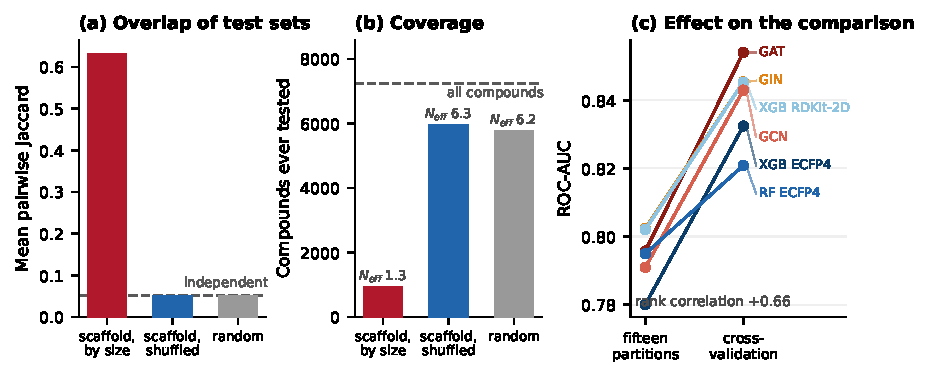
\includegraphics[width=0.98\textwidth]{figures/fig05_design.pdf}
\caption{(a) Overlap between the test sets of fifteen partitions under three schemes. (b)
Compounds ever tested, with the effective number of independent observations. (c) The same
models under the two designs.}
\label{fig:design}
\end{figure}

The cause is our splitter, which orders scaffold groups by descending size before filling the
partitions greedily, so the same large groups reach the training set every time and the test
set is drawn repeatedly from the same pool of small scaffolds. Filling largest-first is not a peculiarity of our code.
The scaffold splitter distributed with DeepChem\cite{deepchem} groups molecules by
Bemis--Murcko scaffold and then splits the groups in decreasing order of size, and the
implementation in DGL-LifeSci\cite{dgllifesci} follows it, placing larger groups before
smaller ones. For a
single partition this is a reasonable way to keep the training set representative. For several
partitions meant to be independent it means the seed governs very little, which is the
quantity measured here. A variant that orders the
groups at random brings the dependence down to the level of independent sampling, giving a
mean Jaccard of $0.052$ against $0.053$ for random splits, $6.32$ effective observations
against $6.24$, and coverage of 5,965 compounds, while remaining scaffold-disjoint.
The defect belongs to the ordering rule, not to scaffold partitioning itself.

It biases the level as well as the independence. Every model scores between $0.026$ and
$0.058$ higher under cross-validation, because the restricted pool from which those test sets
were drawn consists of the smaller and harder scaffolds. The rank correlation between the two
designs is $+0.66$: GAT moves from fourth to first and the random forest from third to last.

Every result above comes from one partition, and that partition was drawn with the rule
Section~\ref{sec:partition} shows to be defective. Applying our own criticism to our own
analysis means redrawing.

Three partitions were drawn with the corrected rule, which shuffles the scaffold groups instead of ordering them by size. Two groups are held out of the shuffle in both rules: the
acyclic compounds, whose Murcko scaffold is the empty string and who number 1,260, and the
largest cyclic group at 1,135. Each exceeds the whole validation or test budget, so placing
either outside training does not give a tenth of the data to test but a sixth of it drawn
from one scaffold; the size-ordered rule sends both to training by construction and the
corrected one is made to do the same. The three test sets share a mean Jaccard of $0.063$
against $0.634$ for the rule that produced the designated partition.

Five GIN models were fitted on each. The difference from the degree ranking on the
ranking AUROC is positive on all three, at $+0.033$, $+0.075$ and $+0.136$, and two
of the three intervals exclude zero (Supporting Information). The direction replicates;
the size does not settle, ranging over a factor of four. Part of that is the number of
models: resampling the twenty of the designated partition down to five widens the mean
interval from $0.073$ to $0.094$, which is most of the gap. The tie fraction carried by the
degree ranking is $0.849$, $0.895$ and $0.905$, against $0.868$ originally, so that finding
does not depend on the partition at all.

Two further observations belong here. The baseline's own agreement varies more across
partitions than any effect this paper reports: $0.536$ to $0.607$, a spread of $0.071$ against
the $0.056$ advantage of the designated partition. A reference assumed rather than measured
would therefore be wrong by more than the quantity it is used to judge, which is the case for
measuring it. And the corrected splitter makes the models look better, not worse: GIN
scores above its designated value on all three partitions and the degree ranking below its own
on two. The defect we identified was working against the models, not for them.


The regime decomposition replicates more cleanly than the aggregate
(Table~\ref{tab:replication_regimes}). A trained GIN exceeds the degree ranking on the
heteroatom alerts and falls below it on the fused aromatic systems, on every partition and
under all three readings of that alert, and every one of the twelve intervals excludes zero.
Whatever else the partition governs, it does not govern this.

\begin{table}[htbp]
\centering
\caption{The regime decomposition on the same three partitions. Entries are the difference between a trained GIN and the degree ranking.}
\label{tab:replication_regimes}
\small
\setlength{\tabcolsep}{4pt}
\begin{tabular}{lccc}
\toprule
Regime & 201 & 202 & 203 \\
\midrule
Heteroatom alerts & +0.479$^{*}$ & +0.246$^{*}$ & +0.622$^{*}$ \\
Fused aromatic (SMARTS) & -0.309$^{*}$ & -0.125$^{*}$ & -0.321$^{*}$ \\
Fused, two or more rings & -0.293$^{*}$ & -0.197$^{*}$ & -0.425$^{*}$ \\
Fused, three or more & -0.180$^{*}$ & -0.146$^{*}$ & -0.317$^{*}$ \\
\bottomrule
\end{tabular}
\begin{flushleft}\footnotesize Every one of the twelve intervals excludes zero, and the sign is the same on every partition and under every reading of the fused-aromatic alert. On the designated partition the two SMARTS regimes give $+0.442$ and $-0.231$.\end{flushleft}
\end{table}


\subsection{Predictive performance}
\label{sec:accuracy}

The graph family leads the classical one by $+0.0146$ ($0.0088$ to $0.0204$) under
scaffold-disjoint cross-validation, but the leading members of the two families differ by
$+0.0088$ and that difference does not survive correction, and removing bond features from a
graph model changes nothing measurable. The advantage is narrow and sits at the edge of what
this design resolves, so we report the comparison as context for the attribution analysis
rather than as a result in its own right. The full ranking, the contrasts and the
hyperparameter search are in the Supporting Information.

\section{Discussion}

\subsection{What a structural baseline changes}

The practice examined here is widespread and reasonable in intent: one shows that a trained
model's attributions agree with known chemistry more closely than chance, or than an untrained
model's, and concludes that the agreement was learned. Neither reference does the work asked
of it. Chance is too weak, since any ranking correlated with molecular structure will beat it,
and a single untrained network is too noisy, since five hundred draws span $0.885$ to $1.275$
and the value obtained depends on a seed.

A model-free structural ranking sits between the two. It is deterministic, so it introduces no
sampling noise; it requires no training, so it costs nothing; and when a trained model fails
to exceed a degree ranking, one knows exactly what it failed to exceed.

The word null would be wrong for it. Atom degree measures substitution and ring fusion, and
the alerts it recovers best are the fused aromatic systems, whose atoms are of high degree
because they are fused: on the lift scale it reaches 31\% of the range attainable under that
regime's own ceiling, which is not the ceiling of the full library, while a trained GIN falls
below chance (Supporting Information). What recommends it is that it needs nothing, no model,
no training, no attribution method and no choice of parameter.

Report agreement on a threshold-free measure and across subsets of the alert library. One
figure at one retained fraction, aggregated over one library, is not an adequate summary: our
own headline changes sign between subsets and changes size with the fraction retained, and a
reader given only the aggregate would conclude that the model adds little, which is not what
the data say. State the decision rule with it, naming which comparisons form a family, what
correction each carries, and where none is applied. Ours is in Section~\ref{sec:rules}, and
writing it down changed two of our own tables.

Report the overlap between the test sets of a design meant to give several observations. A
scheme that looks like fifteen partitions can behave like one: ordering scaffold groups by
size, as the splitter distributed with DeepChem does, gave us an effective $1.26$ observations
from fifteen, and shuffling the groups instead gave $6.32$. The measurement costs nothing and
the remedy is one line.

Where a single comparison is made, make it against a pre-specified model-free structural
ranking instead of chance or a single untrained network, with the panel of alternatives
reported beside it. We suggest atom degree, on the grounds given above, but this is
subordinate to the first recommendation: a model that has demonstrably learned chemistry can
fail an aggregate comparison against the baseline. The baseline is a diagnostic, not a
verdict.

\subsection{Mechanism}

The association between the untrained networks and the degree ranking, $0.57$ once the
shared bound on both is removed, identifies what the untrained baseline has been measuring. Message
passing aggregates over neighbourhoods, gradient magnitude accumulates on atoms with more
neighbours, and the resulting ranking approximates a degree ranking before any learning takes
place. That the association survives training, at a mean Spearman correlation of $0.43$
across the twenty models, shows it is not displaced by what the model learns. That an
untrained network already carries a structural prior is not itself new: random-weight
networks have been shown to extract useful structure in vision,\cite{saxe2011} and the
observation here is the molecular instance of it, with the prior identified as a degree
ranking.

The alternative, that the association is nothing but an artefact of degree being one of the
input features, does not hold: with degree and its valence complement removed, an untrained
network still reproduces the degree ranking under both attribution baselines, at $0.656$ and $0.576$ against $0.682$ and $0.673$ with degree present. Message passing produces the association without
being given the feature. Whether it produces all of it is another matter, and the on-manifold
measurement suggests not; the encoding carries a share that this design does not separate.

Training does modify it, in a direction that can be identified. Regressing the per-molecule change in agreement, trained minus untrained, on three molecular
properties over the 237 evaluation molecules gives $R^2 = 0.49$ with all variance inflation
factors below $2.6$. The predictors are the heteroatom fraction, the spread of atom degree
within the molecule, and the fraction of atoms the alerts cover; all three reach
significance. Training helps more in molecules
with a higher heteroatom fraction ($\beta = +0.79$), less in molecules whose atom degrees vary
widely ($\beta = -0.67$), and less in molecules the alerts already cover extensively
($\beta = -0.42$; all $p < 0.001$). The last is the least comfortable for the account offered
here and we report it as such: where there is most alert to find, training adds least. Training shifts attribution toward
heteroatoms, and it adds least where the degree ranking is already informative.

\subsection{Relation to earlier findings}

Benchmarks with ground-truth rationales have recently been assembled for molecular graphs,
and report that explainers highlight atoms adjacent to the true rationale as a consequence of
message-passing diffusion.\cite{proszewska2025} Our results give the quantitative form of
that observation and name the structural quantity involved. Where \citet{hartog2024} found
alert importance largely model-independent, we quantify how much of that independence
precedes training. The finding of \citet{khasanova2026}, that explanation quality degrades
below a threshold of predictive performance, sits alongside ours without conflict: methods
may agree with one another and with the alerts, and all of them may be delivering what a
trivial structural ranking delivers. That agreement is at most weakly and imprecisely related to performance across
sixty models within a narrow accuracy band is the complement of their result, which concerns
models below that band.

Values above $0.90$ ROC-AUC appear regularly in the Ames literature. Part of the gap to the
$0.82$ to $0.85$ reported here follows from the evaluation, and part from curation: some
studies use the 6,512-compound set of Hansen and co-workers\cite{hansen2009} instead of the 7,255-compound compilation used here. Our own figures are, if anything, generous. The hyperparameter search was not nested
inside the folds, so the out-of-fold estimates are
optimistic in absolute terms and the true gap is wider than reported. Comparisons across
studies should account for all three.

\subsection{Limitations}

Everything here is measured on one endpoint against eighteen SMARTS patterns of our own
encoding, of which fourteen match anything and one supplies 62\% of the alert atoms. Whether
a degree ranking is the right reference for another endpoint, or for a library balanced
differently, these data cannot say; the regime decomposition is the strongest evidence that
the balance matters.

Scaffold grouping shapes both the folds and the evaluation sets. The acyclic compounds form
one group of 1,260 and the largest cyclic group holds 1,135, and dealing scaffolds into ten
folds places each whole, so two folds carry those groups against about 608 compounds for the
rest; the family difference of $+0.0088$ is of the same order as the effect of which fold a
large homogeneous group lands in. Both splitters send the two groups to training, so no
evaluation set here contains an acyclic compound, and the 62\% share of alert atoms carried
by the fused-aromatic pattern falls to 46.5\% over every mutagenic compound the
partial-match rule admits.

The baseline was selected, not fixed in advance, and it is not a null. Atom degree was chosen
on a screen of eleven rankings across three regimes after they were scored, and it carries
real information about this endpoint, so the design does not separate ``the model learned
degree rather than chemistry'' from ``degree is a sufficient statistic for much of this
library''. The screen returned the same ranking on three further partitions. The
pre-specified readings, the eighteen patterns and the retained fraction are fixed in the
released material, which dates them to release, not to a public registration made in advance.

The accuracy comparison is context, not a claim. The hyperparameter search was run once on
the designated partition instead of nested inside the folds, so the out-of-fold estimates are
optimistic in absolute terms; the Supporting Information finds that optimism neither large
enough nor in the right direction to produce the family contrast. Predictions are means over
three training seeds, which removes initialisation noise from the graph models and
contributes nothing to a random forest, so part of the $+0.0146$ contrast is an ensembling
effect, and the intervals hold the fold assignment and the seeds fixed.

The ranking-AUROC decomposition comes from one partition. The regime split replicates in
direction on three partitions drawn with the corrected splitter, but on the lift scale, and
those three carry five models each, not twenty, which widens their intervals by about a
quarter. Two model sets are in play, twenty with stored weights and fifty with stored
overlaps only, and figures from one are not interchangeable with the other.

Three architectures and four attribution methods exhaust neither space. All three are
message-passing networks without learned bond messages, and a directed message-passing
network of the kind introduced by \citet{yang2019} is the obvious extension, which we did
not test; withdrawing bond features from GIN and GAT moves out-of-fold performance by $+0.002$
and $-0.000$, neither resolved, so such a network would have to draw its advantage from
something other than bond information. The mask-based explainer was examined at three
regularisation settings, which does not exhaust its behaviour.

\section{Conclusions}

A trained graph network on the Ames endpoint learns part of the chemistry the alert library
encodes and not another part, and a single aggregate figure reports neither. Against a ranking
by atom degree, which needs no model, GIN is well ahead on the heteroatom-centred alerts and
below chance on the fused aromatic systems; the two effects are of comparable size and
opposite sign, they survive correction, and they hold under three readings of the alert and on
three further partitions. Aggregated over the whole library they cancel.

Two further findings come from the same comparison. Ranking atoms by degree is strong enough
that only one of three architectures beats it, and at the retained fraction this literature
uses none does. That second figure is an artefact of the measure. Most of what a retained fraction selects
from a degree ranking is decided by tie-breaking, and the comparison should be made on the
whole ranking. It does not match every attribution method: TreeSHAP on a
fingerprint model reaches $1.542$, well clear of the baseline, so this is a statement about
message passing and gradients, not molecular attribution at large. A randomly initialised network tracks the degree ranking, the association survives
training in all three architectures and the withdrawal of degree from the input encoding, and
it appears on a second dataset.

Three recommendations follow, set out in full in the Discussion. Report agreement on a
threshold-free measure and across subsets of the alert library rather than as one figure at
one threshold. Report the overlap between the test sets of a multi-partition comparison. And
where a single comparison is made, make it against a pre-specified model-free structural
ranking rather than against chance or an untrained network, and state the decision rule that
governs it.

\section*{Data and Software Availability}

The Ames dataset is publicly available through the Therapeutics Data Commons. The analysis
pipeline, the stored results, the model weights and the fold assignments are available at
\texttt{[repository URL]}, together with the record of which stage produced each result file
and of every quantity quoted in this paper and in the Supporting Information.

\begin{acknowledgement}
The authors thank colleagues at Karamanoğlu Mehmetbey University for comments on an earlier
version of this work.
\end{acknowledgement}

\section*{Author Contributions}
T.K. designed the study, implemented the pipeline, carried out the analyses and drafted the
manuscript. H.Y. supervised the work and revised the manuscript. M.G. contributed to the
design of the evaluation protocol and revised the manuscript. All authors approved the final
version.

\section*{Notes}
The authors declare no competing financial interest.

\begin{suppinfo}
The eighteen SMARTS patterns with per-pattern coverage; data curation, hyperparameter search
budgets and selected configurations; methods in full; pairwise model comparisons and
predictive performance in full; attribution methods on the designated partition; the negative
controls, including the permutation control; the separation of attribution rule from
representation; mask-based explanation under three settings; sensitivity of the untrained
distribution to network size; calibration and conformal coverage; the applicability domain;
the decision rule in full; agreement across architectures and against predictive performance;
the supporting tables from the main analyses; the structural ranking panel on the corrected
partitions; the cost of the non-nested hyperparameter search; three readings of the
fused-aromatic alert; the attribution baseline; the second molecule set; and the ambiguity of
the bit-to-atom map (PDF).
\end{suppinfo}

\bibliography{references}



\end{document}




